\documentclass[12pt,draft]{thesis-umich}

%\input{listingsConfig}
\usepackage{titletoc}
\dottedcontents{subsection}[6.7em]{}{3.2em}{1pc}
\dottedcontents{subsubsection}[8.7em]{}{3.2em}{1pc}
\usepackage{hyperref}
\usepackage{mathtools}
\usepackage{appendix}
\usepackage{titletoc}
\usepackage{amsmath}
\usepackage[format=hang,font={bf}]{caption}
\usepackage{bm}
\usepackage{multirow}
\usepackage{todonotes}
\usepackage{breqn}
\usepackage{subfigure}
\usepackage{enumitem}
\usepackage{tikz}
\usetikzlibrary{shapes,arrows}

% Set up flowchart stuff
\tikzstyle{startstop} = [rectangle, rounded corners, minimum width=3cm, minimum height=1cm,text centered, draw=black, fill=red!30]
\tikzstyle{io} = [trapezium, trapezium left angle=70, trapezium right angle=110, minimum width=2cm, minimum height=1cm, text centered, text width=2cm, draw=black, fill=blue!30]
\tikzstyle{process} = [rectangle, minimum width=3cm, minimum height=1cm, text centered, text width=3cm, draw=black, fill=orange!30]
\tikzstyle{decision} = [diamond, minimum width=3cm, minimum height=1cm, text centered, text width=3cm, draw=black, fill=green!30]
\tikzstyle{arrow} = [thick,->,>=stealth]

% Set up refs
\hypersetup{
    colorlinks,
    citecolor=red,
    filecolor=black,
    linkcolor=black,
    urlcolor=black
}
\setcounter{tocdepth}{4}
\setcounter{secnumdepth}{4}

\newcommand*{\bfrac}[2]{\genfrac{}{}{0pt}{}{#1}{#2}}
\dottedcontents{subsection}[6.0em]{}{2.8em}{1pc}
\dottedcontents{subsubsection}[9.0em]{}{3.5em}{1pc}
% \renewcommand{\thefigure}{\textbf{Figure \arabic{section}}}
% \renewcommand \thesection{\Roman{section}.}rand

\begin{document}

%\titlepage

\pagenumbering{arabic}

\chapter{Introduction}\label{chap:intro}
\ifdraft{
\hl{Need to actually write an introduction}

\begin{itemize}
\item \hl{Introduce two-step/one-step methods}
\item \hl{Talk briefly about rod cusping effects and larger motivations}
\item \hl{Mention what I did}
\end{itemize}
}{}
\todo{punctuate equations correctly and consistently}
\todo{Format equation references appropriately}

\chapter{Neutron Transport Methodology}\label{chap:transport}
\section{Boltzmann Equation}
\todo{Add a chapter intro}

The Boltzmann equation for neutron transport is shown below:

\begin{dmath}\label{e:boltzmann}
{\frac{1}{v} \frac{\partial \psi}{\partial t} + \bm \Omega \cdot \bm \nabla \psi + \Sigma_t\left(\bm x,E,t\right)\psi\left(\bm x,E,\bm \Omega,t\right)} = {\frac{1}{4\pi}\intop_0^{\infty} \intop_{4\pi} \Sigma_s\left(\bm x,E' \rightarrow E, \bm \Omega' \rightarrow \bm \Omega\right) \psi\left(\bm x,E',\bm \Omega'\right) d\Omega' dE'} + {\frac{\chi\left(E\right)}{4\pi} \intop_0^{\infty} \intop_{4\pi} \nu \Sigma_f\left(\bm x,E',t\right) \psi\left(\bm x,E',\bm \Omega,t\right) d\Omega dE' + Q\left(\bm x,E,\bm \Omega,t\right)}
\end{dmath}
\todo{Distinguish between prompt and delayed fission}
\todo{Discuss terms of time-dependent equation, then show steady-state equation}

For many problems, the time dependence of the Boltzmann equation can be neglected.  Doing do eliminates the first term of the equation above.  To ensure neutron balance, this equation is reformulated as an eigenvalue problem.  The eigenvalue $\lambda = \frac{1}{k}$ allows the two sides of the equation to balance.  The cross-sections can then be adjusted until $\lambda = 1$ is achieved, providing a physically meaningful steady-state solution to the equation.  The eigenvalue form of the Boltzmann equation is shown below:

\begin{dmath}\label{e:ssboltzmann}
{\bm \Omega \cdot \bm \nabla \psi + \Sigma_t\left(\bm x,E\right)\psi\left(\bm x,E,\bm \Omega\right) = \frac{1}{4\pi}\intop_0^{\infty} \intop_{4\pi} \Sigma_s\left(\bm x,E' \rightarrow E, \bm \Omega' \rightarrow \bm \Omega\right) \psi\left(\bm x,E',\bm \Omega'\right) d\Omega' dE'} + {\frac{\chi\left(E\right)}{4\pi} \intop_0^{\infty} \intop_{4\pi} \nu \Sigma_f\left(\bm x,E'\right) \psi\left(\bm x,E',\bm \Omega'\right) d\Omega' dE' + \frac{Q\left(\bm x,E,\bm \Omega\right)}{4\pi}}
\end{dmath}
\todo{Use $k_{eff}$ instead of $k$}

Before addressing the methods used to solve equation \ref{e:ssboltzmann}, we will briefly define each of the terms in the equation.  The first term (equation \ref{e:BTEtermsStreaming} is the streaming term.  This describes neutrons with energy $E$ traveling out of the volume dV in the direction $\bm\Omega$.

\begin{equation}\label{e:BTEtermsStreaming}
\bm \Omega \cdot \bm \nabla \psi
\end{equation}

The second term is the total reaction rate (equation \ref{e:BTEtermsTotalRR}).  This describes the total number of collisions experienced in dV by neutrons with energy $E$ and direction $\bm\Omega$.  Equations \ref{e:BTEtermsStreaming} and \ref{e:BTEtermsTotalRR} together make up the total loss of neutrons.

\begin{equation}\label{e:BTEtermsTotalRR}
\Sigma_t\left(\bm x,E\right)\psi\left(\bm x,E\bm\Omega\right)
\end{equation}

Equation \ref{e:BTEtermsScatteringSource} shows the scattering source written in a simplified form.  This is the total number of neutrons scattering into energy $E$ and direction $\bm\Omega$ from all other energies and directions $E'$ and $\bm\Omega'$ in dV.  Because scattering is symmetric around the incident angle, the scattering cross-section depends only on the dot product $\bm\Omega'\cdot\bm\Omega$ rather than each of the two angles independently.

\begin{equation}\label{e:BTEtermsScatteringSource}
\intop_0^{\infty} \intop_{4\pi} \Sigma_s\left(\bm x,E' \rightarrow E, \bm \Omega' \cdot \bm \Omega\right) \psi\left(\bm x,E',\bm \Omega'\right) d\Omega' dE'
\end{equation}

Equation \ref{e:BTEtermsFissionSource} shows neutrons entering dV with energy and direction $E$ and $\bm\Omega$ due to fission.  Fission is an isotropic process, so the total fission source is calculated then distributed evenly across $4\pi$.  Furthermore, the energy distribution of fission is practically independent of incident neutron energy, so the fission neutron distribution $\chi\left(E\right)$ can be outside the integral over energy.

\begin{equation}\label{e:BTEtermsFissionSource}
\frac{\chi\left(E\right)}{4\pi} \intop_0^{\infty} \intop_{4\pi} \nu \Sigma_f\left(\bm x,E,t\right) \psi\left(\bm x,E,\bm \Omega,t\right) d\Omega dE
\end{equation}

Equation \ref{e:BTEtermsExtSource} shows external source term.  This term accounts for all neutrons entering dV with energy and direction $E$ and $\bm\Omega$ from sources other than scatter and fission.  Equation \ref{e:BTEtermsExtSource} shows the source term as a function of angle, but it is often considered to be isotropic like the fission source.

\begin{equation}\label{e:BTEtermsExtSource}
Q\left(\bm x,E,\bm\Omega\right)
\end{equation}

\subsection{Multi-group Approximation}

One important approximation that is commonly made to the transport equation is the multi-group approximation.  To make this approximation, an appropriate energy range for the problem of interest is selected.  This energy range is divided up into $N$ energy groups, with each group going from $E_g$ up to $E_{g-1}$.  For light-water reactor problems, it is common to select 0 eV for $E_N$ and 20 MeV for $E_0$.

We first define the multi-group flux, cross-sections, and chi distribution in equations \ref{e:multigroupDefinitions}.  These definitions ensure that the total reaction rates are preserved in each energy interval $g$.

\begin{subequations}\label{e:multigroupDefinitions}
\begin{equation}\label{e:multigroupangflux}
\psi_g\left(\bm x,\bm \Omega\right)=\frac{1}{E_{n-1}-E_n} \intop_{E_n}^{E_{n-1}} \psi\left(\bm x,E,\bm\Omega\right) dE
\end{equation}
\begin{equation}\label{e:multigroupXS}
\Sigma_{x,g} \psi_g = \frac{1}{E_{n-1}-E_n} \intop_{E_n}^{E_{n-1}} \psi\left(E\right) \Sigma_x\left(E\right) dE \Rightarrow \Sigma_x,g = \frac{\intop_{E_n}^{E_{n-1}} \psi\left(E\right) \Sigma_x\left(E\right) dE}{\intop_{E_n}^{E_{n-1}} \psi\left(E\right) dE}
\end{equation}
\end{subequations}

Using the definitions above, equation \ref{e:ssboltzmann} can be operated on by \ref{e:multigroupIntegral} to obtain the multi-group transport equation \ref{e:multigroupboltzmann}

\begin{equation}\label{e:multigroupIntegral}
\frac{1}{E_{n-1} - E_n}\intop_{E_n}^{E_{n-1}}\left(\cdot\right)dE.
\end{equation}

\begin{dmath}\label{e:multigroupboltzmann}
{\bm \Omega \cdot \bm \nabla \psi_g + \Sigma_{t,g}\left(\bm x\right)\psi_g\left(\bm x,\bm \Omega\right) = \frac{1}{4\pi}\sum_{g'=1}^G \intop_{4\pi} \Sigma_{s,g'\rightarrow g}\left(\bm x,\bm \Omega' \rightarrow \bm \Omega\right) \psi_{g'}\left(\bm x,\bm \Omega'\right) d\Omega'} + {\frac{1}{k}\frac{\chi_g}{4\pi} \sum_{g'=1}^{G} \nu \Sigma_{f,g'}\left(\bm x\right) \intop_{4\pi} \psi_{g'}\left(\bm x,\bm \Omega'\right)d\Omega' + \frac{Q_g\left(\bm x,E\right)}{4\pi}}.
\end{dmath}

\subsection{Discrete Ordinates Approximation}

In addition to energy discretization, it is also useful to discretize the transport equation in angle.  To do this, we use an angular quadrature with angles $\bm\Omega_n$ and associated weights $w_n$:
\todo{More carefully show discretization of polar/azimuthal angles}

\begin{subequations}
\begin{equation}
\sum_{n=1}^N w_n = 4\pi
\end{equation}
\begin{equation}
\sum_{n=1}^N \bm\Omega_n w_n = 0
\end{equation}
\begin{equation}
\intop_{4\pi} f\left(\Omega\right)d\Omega \approx \sum_{n=1}^N f_n w_n
\end{equation}
\end{subequations}

Applying this discretization to the multi-group transport equation \ref{e:multigroupboltzmann}, we obtain the following discrete ordinates (S$_N$) equations:

\begin{dmath}
\bm\Omega_n\cdot\bm\nabla\psi_{g,n} + \Sigma_{t,g}\left(\bm x\right)\psi_{g,n}\left(\bm x\right) = {\frac{1}{4\pi}\sum_{g'=1}^G \sum_{n'=1}^N \Sigma_{g'\rightarrow g,n'\rightarrow n}\left(\bm x\right)\psi_{g',n'}\left(\bm x\right)} + {\frac{1}{k}\frac{\chi_g}{4\pi} \sum_{g'=1}^G \nu\Sigma_{f,g'}\left(\bm x\right)\sum_{n'=1}^N \psi_{g,n}\left(\bm x\right)} + \frac{Q_{g,n}\left(\bm x\right)}{4\pi}
\end{dmath}

\subsection{Diffusion Approximation}

Another approximation that can be made to the angular dependence of the transport equation is the diffusion approximation.  To derive this approximation, we again being with the multi-group transport equation from equation \ref{e:multigroupboltzmann}.  First, we obtain the P$_1$ form of the equation by operating on it by $\intop\left(\cdot\right)d\Omega$ and $\intop\left(\cdot\right)\Omega_i d\Omega$.  To simplify these integrals, we make use of the following identities for integrating over $\bm\Omega$:

\begin{subequations}\label{e:omegaIdentities}
\begin{equation}
\intop_{4\pi} d\Omega = 4\pi
\end{equation}
\begin{equation}
\intop_{4\pi} \Omega_i d\Omega = 0
\end{equation}
\begin{equation}
\intop_{4\pi} \Omega_i\Omega_j d\Omega = \frac{4\pi}{3}\delta_{i,j}
\end{equation}
\begin{equation}
\intop_{4\pi} \Omega_i\Omega_j\Omega_k d\Omega = 0
\end{equation}
\end{subequations}

We must also assume that the angular flux is linearly anisotropic.  This leads to the following expression of the angular flux as a function of the scalar flux $\phi$ and current $J$:

\begin{subequations}
\begin{equation}
\psi_g\left(\bm x,\bm\Omega\right) \approx \frac{1}{4\pi}\left(\phi_g\left(\bm x\right) + 3\bm\Omega \cdot \bm J\left(\bm x\right)\right)
\end{equation}
\begin{equation}
\phi_g\left(\bm x\right) = \intop_{4\pi} \psi_g\left(\bm x,\bm\Omega\right) d\Omega
\end{equation}
\begin{equation}
J_g\left(\bm x\right) = \intop_{4\pi} \psi_g\left(\bm x,\bm\Omega\right) \bm\Omega d\Omega
\end{equation}
\end{subequations}

Applying this assumption and integrating, we obtain a coupled set of four equations for the scalar flux and the three components of the current vector.

\begin{subequations}\label{e:P1transport}
\begin{dmath}\label{e:P1transport-0th}
\frac{d J_x}{dx} + \frac{d J_y}{dy} + \frac{d J_z}{dz} + \Sigma_{t,g}\left(\bm x\right)\phi_g\left(\bm x\right) = {\sum_{g'=1}^G \Sigma_{s0,g'\rightarrow g}\left(\bm x\right)\phi_{g'}\left(\bm x\right)} + {\frac{1}{k}\frac{\chi_g}{4\pi}\sum_{g'=1}^G \nu\Sigma_{f,g'}\left(\bm x\right)\phi_{g'}\left(\bm x\right)} + Q_g\left(\bm x\right)
\end{dmath}
\begin{dmath}\label{e:P1transport-1st-x}
\frac{d\phi_g}{dx} + \Sigma_{t,g}\left(\bm x\right)J_{x,g}\left(\bm x\right)  = {\sum_{g'=1}^G \Sigma_{s1,g'\rightarrow g}\left(\bm x\right) J_{x,g'}\left(\bm x\right)}
\end{dmath}
\begin{dmath}\label{e:P1transport-1st-y}
\frac{d\phi_g}{dy} + \Sigma_{t,g}\left(y\right)J_{y,g}\left(\bm x\right)  = {\sum_{g'=1}^G \Sigma_{s1,g'\rightarrow g}\left(\bm x\right) J_{y,g'}\left(\bm x\right)}
\end{dmath}
\begin{dmath}\label{e:P1transport-1st-z}
\frac{d\phi_g}{dz} + \Sigma_{t,g}\left(\bm x\right)J_{z,g}\left(\bm x\right)  = {\sum_{g'=1}^G \Sigma_{s1,g'\rightarrow g}\left(\bm x\right) J_{z,g'}\left(\bm x\right)}
\end{dmath}
\end{subequations}

Solving equations \ref{e:P1transport-1st-x}-\ref{e:P1transport-1st-z} for the components of the current, we obtain the following expression:

\begin{subequations}\label{e:FicksLaw}
\begin{equation}\label{e:FicksLawCurrent}
\bm J_g\left(\bm x\right) = -D_g\left(\bm x\right) \bm\nabla \phi_g\left(\bm x\right)
\end{equation}
\begin{equation}\label{e:FicksLawDiffConstant}
D_g\left(\bm x\right) = \frac{1}{3}\left(\Sigma_{t,g}-\sum_{g'=1}^G \Sigma_{s1,g'\rightarrow g}\left(\bm x\right)\right)^{-1}
\end{equation}
\end{subequations}

Substituting \ref{e:FicksLawCurrent} into \ref{e:P1transport-0th} gives us the diffusion form of the transport equation, which has only the scalar flux $\phi$ and eigenvalue $\frac{1}{k}$ as unknowns.

\begin{dmath}\label{e:DiffusionEquation}
-\bm\nabla \cdot D_g\left(\bm x\right) \bm \nabla\phi_g\left(\bm x\right) + \Sigma_{t,g}\left(\bm x\right)\phi_g\left(\bm x\right) = {\sum_{g'=1}^G \Sigma_{s0,g'\rightarrow g}\left(\bm x\right)\phi_{g'}\left(\bm x\right)} + {\frac{1}{k}\frac{\chi_g}{4\pi} \sum_{g'=1}^G \nu\Sigma_{f,g'}\left(\bm x\right)\phi_{g'}\left(\bm x\right)} + Q_g\left(\bm x\right)
\end{dmath}

\subsection{Scattering Approximations}

One of the biggest challenges to solving the transport equation is angle dependence of the scattering cross-sections and angular flux.  To simplify the scattering cross-sections, there are two different types of approximations that can be made in MPACT.

\subsubsection{P$_N$ Scattering}

The first scattering approximation that can be made is P$_N$ scattering.  To make this approximation, the $\bm\Omega'\cdot\bm\Omega$ is rewritten as a single angular variable $\mu$, the cosine between the incoming and outgoing scattering angles.  The scattering cross-section can then be expanded in terms of Legendre polynomials, defined by equations \ref{e:LegendrePolynomials}.
\todo{do $\mu_s$ instead of $\mu$}

\begin{subequations}\label{e:LegendrePolynomials}
\begin{equation}
P_{n+1}\left(\bm x\right) = \frac{\left(2n+1\right)xP_n\left(\bm x\right) - nP_{n-1}\left(\bm x\right)}{n+1}
\end{equation}
\begin{equation}
P_0\left(\bm x\right) = 1
\end{equation}
\begin{equation}
P_1\left(\bm x\right) = x
\end{equation}
\begin{equation}
\intop_{-1}^1 P_n\left(\bm x\right) P_m\left(\bm x\right) dx = \frac{2}{2n+1}\delta_{n,m}
\end{equation}
\end{subequations}

Equations \ref{e:PnScatteringExpansion} show the expansion of the scattering cross-section using Legendre polynomials.  Using more terms in the expansion improves the accuracy.  For most reactor problems, $N \le 3$ is sufficient.  Problems such as shielding and others may require many more terms to be kept to obtain sufficient accuracy.

\begin{subequations}\label{e:PnScatteringExpansion}
\begin{equation}
\Sigma_s\left(\bm x,\mu\right) = \sum_{n=0}^N \frac{2n+1}{4\pi} P_n\left(\mu\right) \Sigma_{sn}\left(\bm x\right)
\end{equation}
\begin{equation}
\Sigma_{s,n}\left(\bm x\right) = \intop_{-1}^1 \Sigma_s\left(\bm x,\mu\right) P_n\left(\mu\right) d\mu
\end{equation}
\end{subequations} 

\subsection{Transport Correction}

A second simplification of the scattering source that can be used is transport-corrected isotropic (TCP$_0$) scattering.  When using this approximation, the equation is solved using only the zeroth order term in \ref{e:PnScatteringExpansion}.  The cross-section data used to develop the multi-group scattering cross-sections is modified beforehand to still preserve some of the higher order scattering physics.

Equations \ref{e:outscatterTCP0} show the out-scatter transport correction, which is commonly used in MPACT.  In this correction, the total cross-section and zeroth moment of the self-scatter cross-section are modified by subtracting the sum of the first-order out-scatter data.  There are several variants of the out-scatter correction as well as other completely different correction techniques \todo{Cite for out-scatter, in-scatter, NLC, etc.} that are available in MPACT but will not be discussed in detail here.

\begin{subequations}\label{e:outscatterTCP0}
\begin{equation}
\Sigma_{tr,g} = \Sigma_{t,g} - \sum_{g'=1}^G \Sigma_{s1,g\rightarrow g'}
\end{equation}
\begin{equation}
\Sigma_{s0,g\rightarrow g} = \Sigma_{s0,g\rightarrow g} - \sum_{g'=1}^G \Sigma_{s1,g\rightarrow g'}
\end{equation}
\end{subequations}

\section{Numerical Methods}

A wide variety of numerical methods exist to solve the transport equation, but all of them can be categorized in one of two ways: stochastic (Monte Carlo) or deterministic methods.  Monte Carlo methods use random numbers to directly sample probability distribution functions based on the material cross-sections.  These methods can produce highly accurate, detailed results and make no assumptions about the materials or geometry of the problem.  However, because of the random nature of the method, there is always some uncertainty in the answer.  For large problems, the number of particles that must be simulated to achieve acceptable levels of uncertainty is often too burdensome \ifdraft{\todo{Need a better word}}{} for practical calculations.

All the work discussed in the following sections makes use of deterministic methods.  There are many different deterministic methods, but only the ones relevant to this work will be discussed in the coming sections.

\ifdraft{\subsection{Method of Characteristics}

One method that is commonly used to solve the transport equation is the Method of Characteristics (MOC).  This method allows the transport equation to be solved along a characteristic direction without any approximations, making it useful for complicated geometries, such as those found in nuclear reactors.  To derive this method, the right-hand side of equation \ref{e:ssboltzmann} is replaced by the variable $q$:

\begin{subequations}
\begin{equation}
\bm \Omega \cdot \bm \nabla \psi + \Sigma_t\left(\bm x,E\right)\psi\left(\bm x,E,\bm \Omega\right) = q\left(\bm x,E.\bm \Omega\right)
\end{equation}
\begin{dmath}\label{e:MOCqboltzmann}
{q\left(\bm x,E,\bm \Omega\right) = \intop_{4\pi} \Sigma_s\left(\bm x,E' \rightarrow E, \bm \Omega' \rightarrow \bm \Omega\right) \psi\left(\bm x,E',\bm \Omega'\right) d\bm \Omega'} + {\frac{1}{k}\frac{\chi\left(E\right)}{4\pi} \intop \nu \Sigma_f\left(\bm x,E\right) \psi\left(\bm x,E,\bm \Omega\right) dE + Q\left(\bm x,E,\bm \Omega\right)}
\end{dmath}
\end{subequations}

Now the characteristic direction is introduced:

\begin{equation}
\bm r = \bm {r_0} + s \bm \Omega \Rightarrow \begin{cases} x\left(s\right) = x_0 + s\Omega_x \\ y\left(s\right) = y_0 + s\Omega_y \\ z\left(s\right) = z_0 + s\Omega_z\end{cases}
\end{equation}

Substituting this variable into equation \ref{e:MOCqboltzmann} gives the characteristic form of this equation:

\begin{subequations}
\begin{equation}
\frac{\partial \psi}{\partial s} + \Sigma_t\left(\bm r0_0 + s\bm\Omega,E\right)\psi\left(\bm r0_0 + s\bm\Omega,E,\bm \Omega\right) = q\left(\bm r0_0 + s\bm\Omega,E.\bm \Omega\right)
\end{equation}
\begin{dmath}\label{e:characteristicboltzmann}
{q\left(\bm r0_0 + s\bm\Omega,E,\bm \Omega\right) = \intop_{4\pi} \Sigma_s\left(\bm {r_0} + s \bm\Omega',E' \rightarrow E, \bm \Omega' \rightarrow \bm \Omega\right) \psi\left(\bm {r_0} + s\bm\Omega',E',\bm \Omega'\right) d\bm \Omega'} + {\frac{1}{k}\frac{\chi\left(E\right)}{4\pi} \intop \nu \Sigma_f\left(\bm r0_0 + s\bm\Omega,E\right) \psi\left(\bm {r_0} + s\bm\Omega,E,\bm \Omega\right) dE + Q\left(\bm {r_0} + s\bm\Omega,E,\bm \Omega\right)}
\end{dmath}
\end{subequations}

This equation is easily solved using an integrating factor

\begin{equation}
\exp{-\intop_0^s \Sigma_t\left(\bm {r_0} + s'\bm\Omega,E\right)ds'}
\end{equation}

giving the following solution:

\begin{dmath}\label{e:MOCexact}
{\psi\left(\bm {r_0} + s\bm\Omega,\bm\Omega,E\right) = \psi\left(\bm {r_0},\bm\Omega,E\right)\exp{\left(-\intop_0^s \Sigma_t\left(\bm {r_0} + s'\bm\Omega,E\right)ds'\right)}} + {\intop_0^s q\left(\bm {r_0} + s'\bm\Omega,\bm\Omega, E\right)\exp{\left(-\intop_0^s \Sigma_t\left(\bm {r_0} + s''\bm\Omega,E\right)ds''\right)}ds'}
\end{dmath}

Now if $\bm {r_0}$ is on the boundary of the region of interest, the incoming flux $\psi\left(\bm {r_0},\bm \Omega, E\right)$ is known.  This allows the angular flux to be calculated at any point $s$ to be calculated along the characteristic direction $\bm r$.

Up to this point, no approximations have been made in deriving the method of characteristics.  One approximation that is necessary to use MOC for practical problems is to assume some spatial shape for the source term $q$.  The simplest of these is the flat source approximation.  In this approximation, $q$ is assumed to be flat along $\bm r$.  This simplifies equation \ref{e:MOCexact} to the following:

\begin{dmath}\label{e:MOCflatsource}
\psi\left(\bm {r_0} + s\bm\Omega,\bm\Omega,E\right) = \psi\left(\bm {r_0},\bm\Omega,E\right)\exp{\left(-\intop_0^s \Sigma_t\left(\bm {r_0} + s'\bm\Omega,E\right)ds'\right)} + \cdots
\end{dmath}
% Things to talk about:
%   Flat/linear sources

\subsection{Source Iteration}

Using MOC, fixed source transport problems can be solved.  However, in realistic calculations it is rare that the scattering or fission sources are known.  In order to solve the transport equation for problems with an unknown source distribution, the equation can be re-formulated as follows:
\hl{Insert source iteration form of the equation}

Now making some initial guess for \hl{$\phi^-1$} allows us to solve for \hl{$\phi^0$}.  This process can be repeated for all \hl{$\phi^n$} using the previous iterate \hl{variable$\phi^{n-1}$}.  This method is known as Source Iteration (SI).

Source iteration also has a convenient physical interpretation.  Selecting zero as the initial guess means that the first iterate \hl{$\phi^0$} is simply equal to the sum of sources of new neutrons.  Plugging the expression for \hl{$\phi^0$} into the equation for \hl{$\phi^1$}, we find that the \hl{$\phi^1$} is 

\hl{make sure to talk about how ridiculously slowly it can converge.  Find some references for the math if possible}}{}

\subsection{Coarse-Mesh Finite Difference}\label{ss:CMFD}

The source iteration method provides a convenient way of solving transport problems that guarantees a positive, correct solution.  However, because the source iteration can take hundreds of iterations to converge for typical reactor problems, it is important to accelerate the convergence.  The most common way of doing this is the Coarse-Mesh Finite Difference (CMFD) method.  This method involves solving a diffusion problem on a coarse grid to get the average magnitude of the flux in each coarse cell.  This is then used to scale the flux solution on the fine mesh cells.  In order to ensure consistency between the transport solution and the lower order diffusion solution, coupling coefficients are calculated on the boundaries of the coarse mesh cells to correct the leakage between the cells.

\ifdraft{To derive this method, we begin with equation \hl{diffusion equation} and apply the multigroup approximation:
\hl{multi-group diffusion equation}

\begin{equation}
\end{equation}

Integrating this equation over some volume $V$ and dividing by the total volume creates and equation for the average scalar flux $\overline{\phi}$ in that cell.
\hl{discretized equation}

\begin{equation}
\end{equation}

The boundary conditions for each cell are the currents at the interface between two cells:
\hl{boundary condition equation}

\begin{equation}
\end{equation}

This equation can be determined for each cell in the problem to set up a linear system.  This system can then be solved using one of a variety of standard linear solvers.

Because the currents in the matrix are calculated from the diffusion equation, an inconsistency between the diffusion and transport solutions will arise.  To account for this, current correction factors are calculated at the cell boundaries using the fine mesh transport calculations.  These correction factors are calculated as follows:
\hl{dhat equation}

\begin{equation}
\end{equation}

This defines a relationship between the scalar fluxes on each sides of the interface and the current at the interface.  This relationship allows us to correct the diffusion current that is used in the CMFD matrix:\hl{corrected diffusion current}

\begin{equation}
\end{equation}

\subsection{Simplified Pn}

\hl{I can actually probably get rid of this section completely by just referring to the axial solver as $P_3$ instead of $SP_3$}

\subsection{Power Iteration}



\subsection{Collision Probabilities Method}}{}

\chapter{2D/1D Scheme}\label{chap:2d1d}
\begin{frame}[t]{Background}
    
\begin{itemize}
\begin{columns}
 \begin{column}{0.35\textwidth}
  \item 2D/1D method was developed by researchers at Korea Atomic Energy 
  Research Institute (KAERI) \cite{3DHetWholeCoreTransPlanarMOC,DeCARTTheoryManual,MethodsAndPerformanceOfDecart}
  \begin{itemize}
      \item Takes advantage of reactor geometry
      \item High fidelity transport radially with faster, lower order method axially
  \end{itemize}
\end{column}
\begin{column}{0.55\textwidth}
\includegraphics[width=\columnwidth]{../figs/2d1d-subplane.png}
\vfill  
\end{column}
\end{columns}
\begin{columns}
\begin{column}{0.95\textwidth}
\item Newer 2D/1D code MPACT, jointly developed by University of Michigan and Oak Ridge National Laboratory, is used for this work
\end{column}
\end{columns}
\end{itemize} 
  
\end{frame}

%%%%%%%%%%%%%%%%%%%%%%%%%%%%%%%%%%%%%%%%%%%%%%%%%%%%%%%%%%%%%%%%%%%%%%%%%%%%%%%%%

\begin{frame}[t]{Radial Equations}
    
    \begin{itemize}
      \item Average transport equation axially from $z_{k-\frac{1}{2}}$ to 
      $z_{k+\frac{1}{2}}$
      \item Assume cross sections are axially constant in region of integration
    \end{itemize}
    \begin{dmath*}
        {\Omega_x\frac{\partial \psi_{g}^Z}{\partial x} + 
        \Omega_y\frac{\partial \psi_{g}^Z}{\partial y}} + 
        {\Sigma_{tr,g}\left(x,y\right)\psi_{g}^Z\left(x,y,\bm\Omega\right)} = 
        {q_{g}^Z\left(x,y,\bm \Omega\right)} + 
        {L_{g}^Z\left(x,y,\Omega_z\right)}
    \end{dmath*}
    \begin{dmath*}
        {q_{g}^Z\left(x,y,\bm \Omega\right)} = 
        {\frac{1}{4\pi}\sum_{g'=1}^{G}\intop_{4\pi}\Sigma_{s,g'\rightarrow 
        g}^Z\left(x,y,\bm\Omega'\cdot\bm\Omega\right)\psi_{g'}^Z\left(x,y,\bm\Omega'\right)d\Omega'}
         + {\frac{1}{k_{eff}}\frac{\chi_{g}^Z}{4\pi}\sum_{g'=1}^G\intop_{4\pi} 
        \nu\Sigma_{f,g'}^Z\left(x,y\right)\psi_{g'}^Z\left(x,y,\bm\Omega'\right)d\Omega'}
         + {\frac{Q_{g}^Z\left(x,y\right)}{4\pi}}
    \end{dmath*}
    \begin{align*}
    L_{g}^Z\left(x,y,\Omega_z\right) &= \frac{\Omega_z}{\Delta z_k}\left(\psi_{g,z_{k-\frac{1}{2}}} - \psi_{g,z_{k+\frac{1}{2}}}\right) \approx \frac{J_{g,z_{k-\frac{1}{2}}} - J_{g,z_{k+\frac{1}{2}}}}{4\pi\Delta z_k}
    \end{align*}
    
\end{frame}

%%%%%%%%%%%%%%%%%%%%%%%%%%%%%%%%%%%%%%%%%%%%%%%%%%%%%%%%%%%%%%%%%%%%%%%%%%%%%%%%%

\begin{frame}[t]{Axial Equations}

\begin{itemize}
  \item Average transport equation over x from $x_{i-\frac{1}{2}}$ to 
  $x_{i+\frac{1}{2}}$ and over y from $y_{j-\frac{1}{2}}$ to $y_{j+\frac{1}{2}}$
  \item Assume cross sections are radially constant in region of integration
\end{itemize}
\begin{dmath*}
{\Omega_z \frac{\partial \psi_{g}^{XY}}{\partial z}} + 
{\Sigma_{tr,g}^{XY}\left(z\right)\psi_{g}^{XY}\left(z,\bm\Omega\right)} = 
q_{g}^{XY}\left(z,\bm\Omega\right) + 
{L_{g}^{XY}\left(z,\Omega_x,\Omega_y\right)}
\end{dmath*}
\begin{equation*}
L_{g}^{XY}\left(z,\Omega_x,\Omega_y\right) \approx 
{\frac{J_{g,x_{i-\frac{1}{2}},y_j} - 
  J_{g,x_{i+\frac{1}{2}},y_j}}{4\pi\Delta x_i}} +
\frac{J_{g,x_i,y_{j-\frac{1}{2}}} - J_{g,x_i,y_{j+\frac{1}{2}}}}{4\pi\Delta 
y_j}
\end{equation*}

\end{frame}

%%%%%%%%%%%%%%%%%%%%%%%%%%%%%%%%%%%%%%%%%%%%%%%%%%%%%%%%%%%%%%%%%%%%%%%%%%%%%%%%%

\begin{frame}[t]{Calculation Flow}

\begin{columns}
  \begin{column}{0.6\textwidth}
    \begin{itemize}
      \item 3D CMFD \cite{SmithCMFDOrig}
      \begin{itemize}
        \item Determines global flux shape to scale fine mesh solution
        \item Calculates radial currents for 1D axial solver
      \end{itemize}
      \item 1D NEM-SP$_3$ \cite{SPnEquations,finnemann1977RodCuspingOrigMention}
      \begin{itemize}
        \item Calculates improved axial currents for 2D solver
      \end{itemize}
      \item 2D MOC \cite{AskerMOCOrig1972,HalsallMOCOrigCACTUS1980}
      \begin{itemize}
        \item Solves for fine mesh scalar flux
        \item Calculates updated radial currents for CMFD calculation
      \end{itemize}
    \end{itemize}
  \end{column}
\begin{column}{0.4\textwidth}
  \begin{figure}[h]
    \centering
    \resizebox{!}{0.7\textheight}{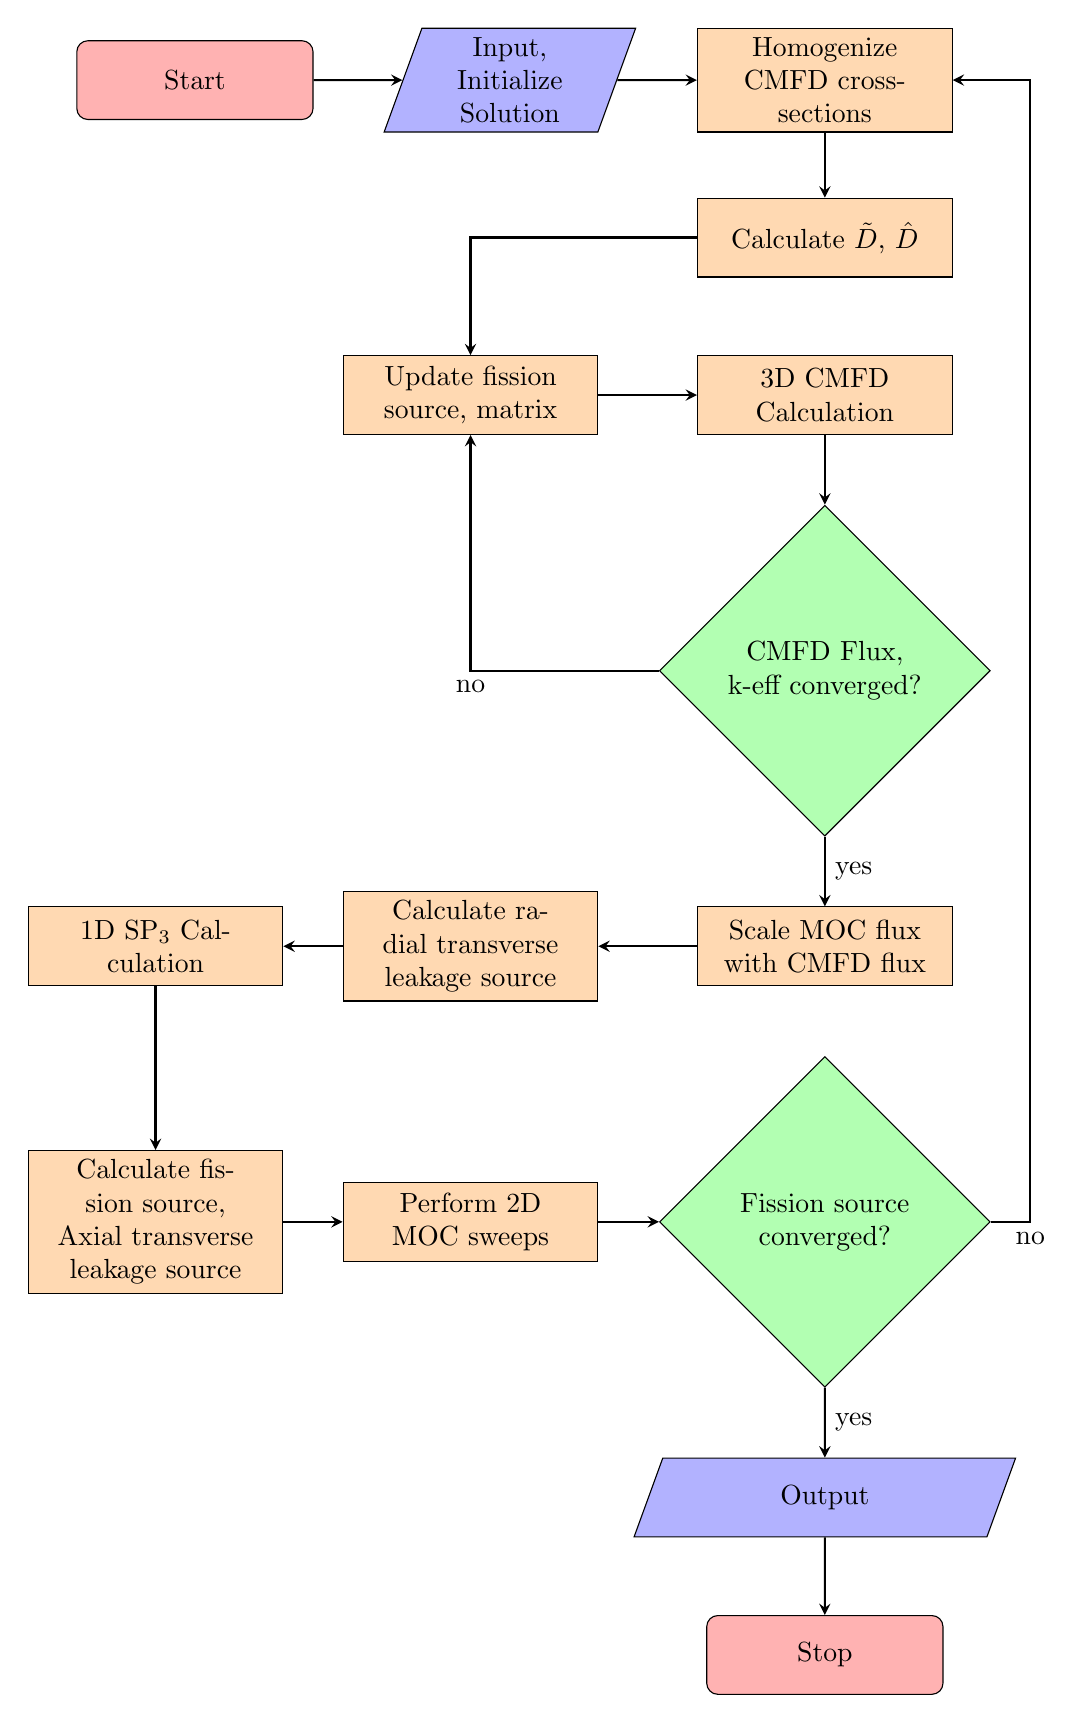
\begin{tikzpicture}[node distance=2cm]

% Begin
\node (start) [startstop] {Start};
\node (init) [io, right of=start, xshift=2.0cm] {Input, Initialize Solution};

% CMFD
\node (homog) [process, right of=init, xshift=2.0cm] {Homogenize CMFD cross-sections};
\node (calcCouplingCoeffs) [process, below of=homog] {Calculate $\tilde{D}$, $\hat{D}$};
\node (3DCMFD) [process, below of=calcCouplingCoeffs] {3D CMFD Calculation};
\node (CMFDupdate) [process, left of=3DCMFD, xshift=-2.5cm] {Update fission source, matrix};
\node (CMFDconv) [decision, below of=3DCMFD, yshift=-1.5cm] {CMFD Flux, k-eff converged?};
\node (proj) [process, below of=CMFDconv, yshift=-1.5cm] {Scale MOC flux with CMFD flux};

% Nodal
\node (radialTL) [process, left of=proj, xshift=-2.5cm] {Calculate radial transverse leakage source};
\node (sp3) [process, left of=radialTL, xshift=-2.0cm] {1D SP$_3$ Calculation};

% MOC
\node (axialTL) [process, below of=sp3,yshift=-1.5cm] {Calculate fission source, Axial transverse leakage source};
\node (MOC) [process, right of=axialTL, xshift=2.0cm] {Perform 2D MOC sweeps};
\node (MOCconv) [decision, right of=MOC,xshift=2.5cm] {Fission source converged?};
\node (output) [io, below of=MOCconv,yshift=-1.5cm] {Output};
\node (stop) [startstop, below of=output] {Stop};

% Basic Arrows
\draw [arrow] (start) -- (init);
\draw [arrow] (init) -- (homog);
\draw [arrow] (homog) -- (calcCouplingCoeffs);
\draw [arrow] (calcCouplingCoeffs) -| (CMFDupdate);
\draw [arrow] (CMFDupdate) -- (3DCMFD);
\draw [arrow] (3DCMFD) -- (CMFDconv);
\draw [arrow] (CMFDconv) -- node[anchor=west] {yes} (proj);
\draw [arrow] (proj) -- (radialTL);
\draw [arrow] (radialTL) -- (sp3);
\draw [arrow] (sp3) -- (axialTL);
\draw [arrow] (axialTL) -- (MOC);
\draw [arrow] (MOC) -- (MOCconv);
\draw [arrow] (MOCconv) -- node[anchor=west] {yes} (output);
\draw [arrow] (output) -- (stop);

% Fancy Arrows
\draw [arrow] (CMFDconv) -| node[anchor=north] {no} (CMFDupdate);
\draw [arrow] (MOCconv) -| node[anchor=north] {no} ([xshift=0.5cm]CMFDconv.east) |- (homog);

\end{tikzpicture}}
  \end{figure}
\end{column}
\end{columns}

\end{frame}

%%%%%%%%%%%%%%%%%%%%%%%%%%%%%%%%%%%%%%%%%%%%%%%%%%%%%%%%%%%%%%%%%%%%%%%%%%%%%%%%%

\begin{frame}[t]{3D CMFD}
    
        \begin{itemize}
          \item Diffusion-based acceleration performed on coarse mesh
          \item $\hat{D}$ coupling coefficients enforce consistency between diffusion and transport solutions
          \begin{equation*}\scriptstyle
          \hat{D}_{g,s} = \frac{J_{g,s}^{trans,k-1} + 
            \tilde{D}_{g,s}\left(\phi_{g,p}^{diff,k} - 
            \phi_{g,m}^{diff,k}\right)}{\left(\phi_{g,p}^{trans,k} + 
            \phi_{g,m}^{diff,k}\right)}
          \end{equation*}
          \item Coarse mesh solution projected to fine mesh solution, preserving MOC radial shape and CMFD volume-averaged flux
          \begin{equation*}\scriptstyle
          \phi_{g,j}^{MOC,k} = \frac{\phi_{g,i}^{CMFD,k}}{\phi_{g,i}^{CMFD,k-1}} \phi_{g,j}^{MOC,k-1}
          \end{equation*}
          \item Subplane scheme is used to capture subplane axial flux shapes
        \end{itemize}
    
\end{frame}

%%%%%%%%%%%%%%%%%%%%%%%%%%%%%%%%%%%%%%%%%%%%%%%%%%%%%%%%%%%%%%%%%%%%%%%%%%%%%%%%%

\begin{frame}[t]{1D SP$_3$-NEM}
    
    \begin{columns}
      \begin{column}{0.6\textwidth}
        \begin{itemize}
          \item SP$_3$ \cite{SPnEquations} used to handle angular shape 
          \begin{dmath*}\scriptstyle
            {-\bm{\nabla} \cdot D_{0,g} \left(\bm x\right) \bm \nabla 
            \Phi_{0,g}\left(\bm x\right) + \left[\Sigma_{tr,g}\left(\bm 
            x\right) - \Sigma_{s0,g}\left(\bm 
            x\right)\right]\Phi_{0,g}\left(\bm x\right)} = {Q_g\left(\bm 
            x\right) + 2\left[\Sigma_{tr,g}\left(\bm x\right) - 
            \Sigma_{s0,g}\left(\bm x\right)\right]\Phi_{2,g}\left(\bm 
            x\right)}
          \end{dmath*}
          \begin{dmath*}\scriptstyle
            {-\bm{\nabla} \cdot D_{2,g} \left(\bm x\right) \bm \nabla 
            \Phi_{2,g}\left(\bm x\right) + \left[\Sigma_{tr,g}\left(\bm 
            x\right) - \Sigma_{s2,g}\left(\bm 
            x\right)\right]\Phi_{2,g}\left(\bm x\right)} = 
            {\frac{2}{5}\left\lbrace \left[\Sigma_{tr,g}\left(\bm x\right) - 
            \Sigma_{s0,g}\left(\bm x\right)\right]\left[\Phi_{0,g}\left(\bm 
            x\right) - 2\Phi_{2,g}\left(\bm x\right)\right] - Q_g\left(\bm 
            x\right) \right\rbrace}
          \end{dmath*}
          \item NEM \cite{finnemann1977RodCuspingOrigMention} used to handle spatial shape
          \begin{equation*}\scriptstyle
          Q\left(\xi\right) = \sum_{i=0}^2 q_i P_i\left(\xi\right)\ , \quad 
          \phi\left(\xi\right) = \sum_{i=0}^4 \phi_i P_i\left(\xi\right)
          \end{equation*}
          \begin{equation*}\scriptstyle
          \intop_{-1}^1 P_n\left(\xi\right) 
          \left(-\frac{D}{h^2}\frac{d^2}{d\xi^2}\phi\left(\xi\right) + \Sigma_r 
          \phi\left(\xi\right) - Q\left(\xi\right)\right)d\xi = 0,\ n=0,1,2
          \end{equation*}
          \begin{equation*}\scriptstyle
          \phi_L\left(1\right) = \phi_R\left(-1\right)\ , \quad 
          J_L\left(1\right) = J_R\left(-1\right)
          \end{equation*}
        \end{itemize}
      \end{column}
    \begin{column}{0.4\textwidth}
      \begin{figure}[h]
        \centering
        \resizebox{!}{0.5\textheight}{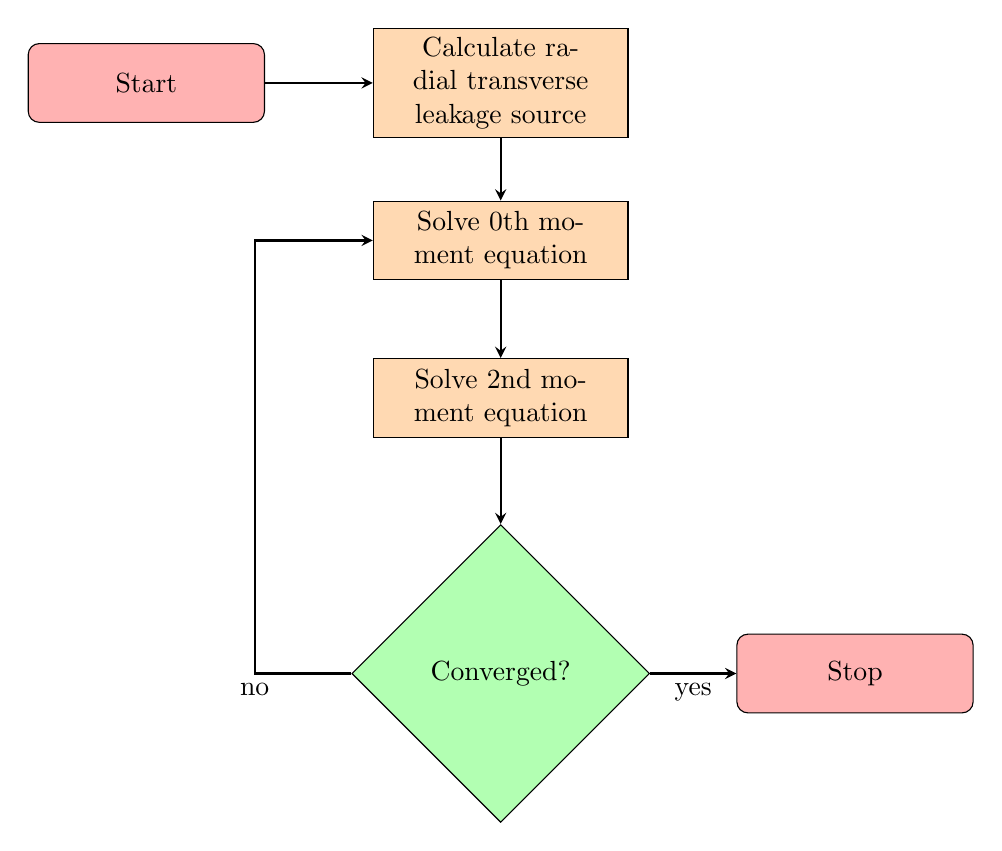
\begin{tikzpicture}[node distance=2cm]

% Begin
\node (start) [startstop] {Start};

% Nodal
\node (radialTL) [process, right of=start, xshift=2.5cm] {Calculate radial transverse leakage source};
\node (sp3-0) [process, below of=radialTL] {Solve 0th moment equation};
\node (sp3-2) [process, below of=sp3-0] {Solve 2nd moment equation};
\node (convCheck) [decision, below of=sp3-2, yshift=-1.5cm] {Converged?};

% Stop
\node (stop) [startstop, right of=convCheck, xshift=2.5cm] {Stop};

% Basic Arrows
\draw [arrow] (start) -- (radialTL);
\draw [arrow] (radialTL) -- (sp3-0);
\draw [arrow] (sp3-0) -- (sp3-2);
\draw [arrow] (sp3-2) -- (convCheck);
\draw [arrow] (convCheck) -- node[anchor=north] {yes} (stop);

% Fancy Arrows
\draw [arrow] (convCheck) -| node[anchor=north] {no} ([xshift=-1.5cm]sp3-2.west) |- (sp3-0);

\end{tikzpicture}}
      \end{figure}
    \end{column}
    \end{columns}
    
\end{frame}

%%%%%%%%%%%%%%%%%%%%%%%%%%%%%%%%%%%%%%%%%%%%%%%%%%%%%%%%%%%%%%%%%%%%%%%%%%%%%%%%%

\begin{frame}[t]{2D MOC}

    \begin{itemize}
      \item Solve along a specific direction $\Omega_n$ to reduce the problem from a PDE to an ODE that can be solved analytically
      \begin{equation*}\scriptstyle
      \frac{\partial \psi_{g,n}}{\partial s} + \Sigma_{t,g}\left(\bm r_0 + 
      s\bm\Omega_n\right)\psi_{g,n}\left(\bm r_0 + s\bm\Omega_n\right) = 
      q_{g,n}\left(\bm r_0 + s\bm\Omega_n\right)
      \end{equation*}
      \begin{dmath*}\scriptstyle
        {\psi_{g,n}\left(\bm r_0 + s\bm\Omega_n\right) = \psi_{g,n}\left(\bm 
        r_0\right)\exp{\left(-\intop_0^s \Sigma_{t,g}\left(\bm r_0 + 
        s'\bm\Omega_n\right)ds'\right)}} + {\intop_0^s q_{g,n}\left(\bm r_0 + 
        s'\bm\Omega_n\right)\exp{\left(-\intop_0^{s'} \Sigma_{t,g}\left(\bm r_0 
        + s''\bm\Omega_n\right)ds''\right)}ds'}
      \end{dmath*}
  \item Assume flat source, cross section along track with 
length $L_j$ and spacing $\delta x$
\begin{align*}\scriptstyle
\psi^{out}_{g,i,n,j} &\scriptstyle = \psi^{in}_{g,i,n,j}e^{-\Sigma_{t,g,i} 
    L_j} + \frac{q_{g,i,n}}{\Sigma_{t,g,i}}\left(1 - 
e^{-\Sigma_{t,g,i}L_j}\right) \\\scriptstyle
\overline{\psi}_{g,i,n,j} &\scriptstyle = 
\frac{q_{g,n,i}}{\Sigma_{t,g,i}} + \frac{1 - e^{-\Sigma_{t,g,i} 
        L_j}}{L_j\Sigma_{t,g,i}}\left(\psi^{in}_{g,i,n,j} - 
\frac{q_{g,n,i}}{\Sigma_{t,g,i}}\right) \\\scriptstyle
\overline{\psi}_{g,i,n} &\scriptstyle = \frac{\sum_j 
    \overline{\psi}_{g,i,n,j} \delta x L_j}{\sum_j \delta x L_j}
\end{align*}
    \end{itemize}

\end{frame} 

%%%%%%%%%%%%%%%%%%%%%%%%%%%%%%%%%%%%%%%%%%%%%%%%%%%%%%%%%%%%%%%%%%%%%%%%%%%%%%%%%

\begin{frame}[t]{2D MOC}
  
  \begin{columns}
    \begin{column}{0.55\textwidth}
      \begin{itemize}
        \item Perform ray tracing and store segment information up front
        \item Set up scattering, fission, and axial transverse leakage sources
        \begin{itemize}
            \item Multi-group sweeping
          \item 1-group sweeping
        \end{itemize}
        \item Parallel Decomposition
        \begin{itemize}
          \item Spatial (Planar and Radial)- MPI
          \item Angle - MPI
          \item Ray - OpenMP
        \end{itemize}
      \end{itemize}
    \end{column}
    \begin{column}{0.45\textwidth}
      \includegraphics[width=\columnwidth]{modular_rays.png}
    \end{column}
  \end{columns}

\end{frame}

\chapter{Rod Cusping}\label{chap:cusping}
This chapter will focus specifically on control rod cusping effects, which are the focus of this work.  First, a more thorough definition of the problem and motivation for solving it will be presented.  The next section will then present some of the solutions that have been used to minimize the cusping effects in the past, including a simplified decusping model implemented in MPACT itself.  The third section will then discuss some newer methods based on the sublpane CMFD scheme that have recently been implemented in MPACT.  Finally, a new ``sub-ray'' MOC method will be proposed to deal with the cause of the cusping effects on a more fundamental level.

\section{Background}

In Section \todo{section num}, some potential sources of errors for the 2D/1D scheme were introduced.  One of these was the error introduced by axial homogenization within a 2D MOC plane.  In some cases, this can be done without introducing significant errors.  For example, MPACT often homogenizes components outside the active fuel region, such as the end plugs and gaps at the end of the fuel rods.  However, when strong neutron absorbers, such as control rods, are homogenized axially in active fuel region, this has the effect of introducing absorption in regions where there should be none.  This effect is known as ``cusping,'' and is illustrated in Figure 

\begin{figure}
    \centering
    \includegraphics[width=0.4\textwidth]{figs/cusping_effect_Joo.png}
    \caption{Illustration of Rod ``Cusping''}\label{f:cuspingEffectJoo}
\end{figure}
\todo{cite}

In some cases, this is easily handled by setting up an appropriate axial mesh which prevents the need for the homogenization, but this is not always a practical solution.  Throughout the course of an entire cycle of operation (usually about 18 months), several different control banks in the reactor may move to a variety of positions to maintain criticality in the core.  Control rods in a PWR typically have step sizes of approximately 1.5 cm, but a typical MOC plane in MPACT is about 8 cm thick in the active fuel region.  In order to prevent cusping effects for an entire cycle, the user may have to create a very detailed axial mesh to ensure that all the control rod positions used throughout the cycle align with the edge of an MOC plane.  Not only is this tedious for the user, but it also greatly increases the computational burden due to the increased number of MOC planes.  Figure \ref{f:p4cuspingEffects} shows the calculated k-eff as a function of control rod position.  The cusping effects in this figure are further complicated by a heterogeneous rod with AIC and B$_4$C poison regions and a stainless steal tip.  Thus, cusping effects occur not just at the control rod tip, but also at material interfaces throughout the rod.

\begin{figure}
    \centering
    \includegraphics[width=0.8\textwidth]{figs/p4cuspingEffects.png}
    \caption{Control Rod Cusping Effects for 3x3 Assembly}\label{f:p4cuspingEffects}
\end{figure}

\section{Traditional Solutions}

\subsection{Nodal Codes}

\hl{Discuss ways people have addressed this in the past}

\subsection{2D/1D Codes}

Several codes that have employed the 2D/1D method in recent years have also required rod decusping methods.  MPACT currently uses a simple polynomial correction to the volume fractions used to homogenize the control rod\todo{cite Brendan m\& C 2015}.  To develop this method, a 3x3 assembly was set up with a control rod in the center assembly.  This problem was simulated with the rod tip at nine different positions in the plane.  These simulations were then repeated, but with the axial mesh refined so the rod tip aligned with a plane boundary.  The k-eff differences between the two sets of simulations were fitted with a sixth-order polynomial which is used in MPACT to reduce the volume fraction of the control rod by an appropriate amount to offset the cusping effects.  This process was repeated for different control rod materials such as AIC, B$_4$C, and Tungsten, since each material has unique cross-sections.  This method has the advantages of being simple to implement and requiring no increase in computational requirements.  However, the results obtained from this decusping method are tied to the control rod material and reactor model used to develop the corrections, limiting its usefulness to a small subset of reactors.

Another 2D/1D code is nTRACER, which is under active development by \hl{some people in Korea}.  To address rod cusping effects in nTRACER, \hl{Korean guy}, et al. developed a more general method than the polynomial correction method used by MPACT\todo{cite ICAPPS}.  This method pre-generates correction factors at the start of a simulation, rather than relying on hard-coded corrections.  To do this, the assembly that will have a partially inserted control rod is identified, and a single-plane 3x3 assembly problem is set up using the partially-rodded assembly and its neighbors.  The radial and axial cusping effects are then determined separately.  First, the radial cusping effects are determined by performing 2D MOC calculations on the 3x3 sub-domain with the rod fully inserted and fully withdrawn.  This provides radial flux profiles in the rodded assembly for both rodded and unrodded regions, as well as current coupling coefficients for CMFD for the rodded and unrodded CMFD nodes.  Once this is done, the rod is simulated at positions of 25\%, 50\%, and 75\% withdrawn from the plane.  To reduce runtime, these calculations are done using only 3D sub-plane CMFD.  This generates axial flux profiles for the full MOC plane for each of the possible rod positions.  During the full-core 2D/1D calculation, these axial flux profiles are then used to generate improved homogenized cross-sections for the MOC calculation using equation \ref{e:nTRACERdecusping}.

\begin{equation}\label{e:nTRACERdecusping}
\overline{\Sigma_i} = \frac{\phi_{rad,i}^R \phi_{ax,i}^R \Sigma_i^R h^R + \phi_{rad,i}^U \phi_{ax,i}^U \Sigma_i^U h^U}{\phi_{rad,i}^R \phi_{ax,i}^R h^R + \phi_{rad,i}^U \phi_{ax,i}^U h^U}
\end{equation}

\hl{DeCART?  Other 2D/1D codes?}

\section{Improved Decusping Methods}
\todo{Better Title?  Not that much ``better''}

This section discusses two new decusping treatments added to MPACT.  These methods rely on the sub-plane scheme described in section \todo{ref}.  The first method only treats the axial cusping effects, while the second method extends the first by also treating the radial decusping effects.

\subsection{Subplane Decusping}

\todo{Does this really belong anywhere?}

\begin{table}
\caption{Comparison of MPACT and DeCART subplane scheme results for C5G7-like rodded problem}
\begin{center}
\begin{tabular}{|l|c|c|c|c|c|c|}\hline
Plane & \multicolumn{2}{|c|}{k-eff Diff.} & \multicolumn{2}{|c|}{Max Power Diff.} & \multicolumn{2}{|c|}{Relative Runtime} \\ \cline{2-7}
Division & MPACT & DeCART & MPACT & DeCART & MPACT & DeCART \\ \hline
2 & 0.6 & 5.2 & 0.003\% & 0.04\% & 0.579 & 0.513 \\ \hline
3 & 1.9 & 7.7 & 0.004\% & 0.10\% & 0.408 & 0.327 \\ \hline
5 & 2.2 & 9.5 & 0.008\% & 0.11\% & 0.350 & 0.214 \\ \hline
10 & 1.2 & 9.8 & 0.020\% & 0.22\% & 0.253 & 0.058 \\ \hline
\end{tabular}
\end{center}
\end{table}

\begin{table}
\caption{Comparison of subplane scheme to traditional 2D/1D for VERA Progression Problem 4}
\begin{center}
\resizebox{\textwidth}{!}{\begin{tabular}{|l|c|c|c|c|c|c|c|c|}\hline
Number & k-eff Diff. & \multicolumn{2}{|c|}{Power Diff.} & \multicolumn{2}{|c|}{Outer Iterations} & \multicolumn{3}{|c|}{Runtime (core-hours)} \\\hline
of Planes & (pcm) & RMS & Max & Traditional & Subplane & Traditional & Subplane & Ratio ($\frac{Subplane}{Traditional}$) \\\cline{3-9}
32 & 0.01 & 0.001\% & 0.004\% & 29 & 30 & 21.0 & 16.2 & 0.77 \\\hline
46 & 0.01 & 0.018\% & 0.053\% & 14 & 21 & 10.3 & 8.9 & 0.86 \\\hline
62 & 0.04 & 0.023\% & 0.056\% & 12 & 20 & 12.4 & 11.5 & 0.93 \\\hline
77 & 0.04 & 0.022\% & 0.067\% & 12 & 21 & 13.0 & 11.4 & 0.88 \\\hline
\end{tabular}}
\end{center}
\end{table}

\begin{table}
\caption{Comparison of subplane scheme to traditional 2D/1D for VERA Progression Problem 5}
\begin{center}
\resizebox{\textwidth}{!}{\begin{tabular}{|l|c|c|c|c|c|c|c|c|}\hline
Number & k-eff Diff. & \multicolumn{2}{|c|}{Power Diff.} & \multicolumn{2}{|c|}{Outer Iterations} & \multicolumn{3}{|c|}{Runtime (core-hours)} \\\hline
of Planes & (pcm) & RMS & Max & Traditional & Subplane & Traditional & Subplane & Ratio ($\frac{Subplane}{Traditional}$) \\\cline{3-9}
32 & 0.01 & 0.004\% & 0.008\% & 28 & 29 & 996  & 1325 & 1.33 \\\hline
46 & 0.11 & 0.044\% & 0.111\% & 13 & 29 & 691  & 829  & 1.20 \\\hline
62 & 0.07 & 0.028\% & 0.190\% & 12 & 46 & 880  & 918  & 1.04 \\\hline
77 & 0.08 & 0.030\% & 0.184\% & 12 & 45 & 1090 & 1013 & 0.93 \\\hline
\end{tabular}}
\end{center}
\end{table}

\subsection{Auxiliary 1D Collision Probabilities}

The CMFD homogenized flux can be calculated as follows:

\begin{equation}\label{e:CMFDsubplaneFlux}
\phi^k_{g,c} = \frac{\sum_{i=1}^{N_{FSR}} \phi^{k=1}_{g,i} V_i}{\sum_{i=1}^{N_{FSR}} V_i} c_{g,c}
\end{equation}

The subscripts $i$, $g$, and $c$ are fine mesh cell indexes, energy group indexes, and CMFD cell indexes, respectively.  The factor $c_{g,c}$ is a group- and cell-dependent scaling factor for the subplane method.  This factor provides an axial shape to the MOC flux using the previous iterate.  It is defined as follows:

\begin{equation}\label{e:CMFDsubplaneFactor}
c_{g,c} = \frac{\phi^{k-1}_{g,c}}{\overline{\phi^k_{g,c}}}
\end{equation}

where the average flux in the denominator is defined by

\begin{equation}\label{e:CMFDaverageFlux}
\phi^k_{g,c} = \frac{\sum_{i=1}^{N_{FSR}} \phi^{k=1}_{g,i} V_i}{\sum_{i=1}^{N_{FSR}} V_i}
\end{equation}

This definition of the subplane factor provides axial shape while still preserving the volume-averaged flux and reaction rates in each pin cell in the MOC plane.

The CMFD homogenized cross-sections can be calculated using the MOC flux:

\begin{equation}\label{e:CMFDhomXS}
\Sigma_{x,c} = \frac{\sum_{i=1}^{N_{FSR}} \phi_{g,i}\Sigma_{x,g,i}V_i}{\sum_{i=1}^{N_{FSR}} \phi_{g,i}V_i}
\end{equation}

Multiplying equations \ref{e:CMFDsubplaneFlux} and \ref{e:CMFDhomXS} gives the reaction rate in the pin cell.

When using the embedded solver, a radial flux profile is obtained from the solver.  The process described above is followed for the nodes around the partially inserted rod.  However, instead of the MOC flux, the radial flux from the embedded solver is used.  This allows subplanes with partially inserted control rods to have different cross-sections based on the radial flux profile around the tip of the control rod.

\hl{The flux coming out of the embedded solver is treated as a shape function and scaled to preserve the MOC flux.}

\hl{Need to make sure reaction rates are preserved I think}.

\hl{A constant current is used for all subplanes.  This does not provide the most accurate solution, but ensures stability and neutron balance.}

\hl{When projecting, the subplane fluxes scale MOC fluxes.  Reference equation.}

\hl{The cross-sections can be modified by mixing the rodded and unrodded cross-sections.  Equation from Han Joo cusping paper.}

\section{Future Work}

\subsection{Auxiliary Solver}

\hl{Something better than 1D CPM... Namely MOC}

\subsection{Radial Transverse Leakage Source}

\hl{sub-plane dependent dhats/currents}

\subsection{Axial Transverse Leakage Source}

\hl{Spatially dependent axial TL}

\subsection{Sub-Ray MOC}

\hl{Boom}

\chapter{Results}\label{chap:results}
To test MPACT's newly developed decusping methods, VERA Progression Problems 4 and 5 \cite{VERAProgressionProblems} were used.  These problems are based on Watts Bar Unit 1, and provide realistic test cases for the 2D/1D method.  The control rods and meshing were modified slightly from the specifications to introduce rod cusping effects which may not normally be there.  However, these changes will be useful in identifying the effects of cusping and improvements from each decusping method for each of the two different problems.

\section{VERA Problem 4}

Problem 4 is composed of a 3x3 set of assemblies, with a control bank in the center assembly.  The radial layout of the problem is shown in Figure \ref{f:p4radial}, and the axial layout of each assembly is shown in Figure \ref{f:p4axial}.  The control rods were placed at an axial elevation of 257.9 cm above the core plate, about one third inserted into the core.  The rod in the original problem specification is made of AIC with a B$_4$C follower and a stainless steel tip.  However, to simplify analysis of the results, this was changed so the rod was a single AIC region.

For the reference solution, 58 MOC planes were used.  It was also ensured that the end of the control rods were exactly aligned with one of the MOC plane boundaries.  The cases using decusping methods used the same mesh, but with the 2 MOC planes around the tip of the control rod merged into a single plane to introduce cusping effects.  The accuracy and convergence data for these cases are shown in Table \ref{t:p4decusp}

\begin{figure}[h]\label{f:p4layout}
\centering
\subfigure{\label{f:p4radial}
\includegraphics[width=0.4\textwidth]{p4a_layout.png}
}
~
\subfigure{\label{f:p4axial}
\includegraphics[width=0.3\textwidth]{wb_3d_assembly.png}
}
\caption{VERA Problem 4 radial (left) and axial (right) layouts}\label{f:p4}
\end{figure}

\begin{table}[h]
\centering
\caption{VERA Problem 4 Decusping Results}\label{t:p4decusp}
\resizebox{\textwidth}{!}{
\begin{tabular}{|c|c|c|c|c|c|c|}\hline
\multirow{2}{*}{Case} & k-eff & \multicolumn{2}{|c|}{Pin Power Differences} & \multicolumn{2}{|c|}{Iterations} & Runtime\\\cline{3-6}
 & Difference (pcm) & RMS & Max & 2D/1D & CMFD & (Core-Hours) \\\hline
Reference        & -- & --     & --      & 12 & 364 & 8.59 \\\hline
No Treatment     & -30 & 3.84\% & 21.81\% & 12 & 352 & 9.23 \\\hline
Polynomial       & -8  & 1.03\% &  6.58\% & 12 & 360 & 9.50 \\\hline
Sub-plane         & -7  & 1.13\% &  7.11\% & 12 & 409 & 9.26 \\\hline
Sub-plane + 1D-CP & -2  & 0.54\% &  4.94\% & 12 & 364 & 9.45 \\\hline
\end{tabular}
}
\end{table}

The ``No Treatment'' case shows the magnitude of the cusping effects for this problem.  The k$_{eff}$ difference is 30 pcm, which is not too alarming.  However, the RMS and maximum power differences are almost 4\% and over 20\%, respectively, which is an unacceptable level of error.  The polynomial decusping significantly reduces these errors to about 1\% and 6.5\% respectively.  This is much better, but still quite high.  The sub-plane decusping with no radial treatment performs similarly to the polynomial decusping, but slightly worse.  Because the polynomials were generated using this problem, it is expected that they would perform well.  Thus, the fact that the sub-plane decusping is comparable indicates that it is capturing the axial shape well.  Finally, the CP-based decusping gives the best results, with an RMS of about 0.5\% and a maximum error just under 5\%.  The maximum error is still larger than what is typically desired from the 2D/1D method, but is better than the old decusping treatment and far better than no treatment at all.

As far as runtime is convergence and runtime is concerned, all cases took the same number of 2D/1D iterations.  The sub-plane--based decusping methods incurred a few more CMFD iterations, but this did not have a significant impact on runtime.  The difference in runtime between the reference and no treatment cases is due to the decomposition of the problem.  Both cases use the same sub-plane CMFD mesh (with homogeneous cross-sections in each plane).  However, the reference case was run with two MOC planes instead of one.  This also means that an extra core was used in the calculation.  Because of this, the time required for the transport calculations was the same, but the CMFD solve was slower for the no treatment case since a single core was solving a portion of the CMFD system handled by two cores in the reference calculation.  Thus, the runtime increase is due only to the parallel partitioning, not the methods themselves.  This is important, because the runtimes of the decusping cases were all about the same as the no treatment case.  This implies that the runtime penalty due to the decusping solvers is negligible.  Some work simply needs to be done to improve the parallel balance when using the sub-plane scheme.

\section{VERA Problem 5}

To demonstrate the behavior of the decusping methods on a full-core problem, VERA Problem 5 was also run.  Problem 5 is the a beginning-of-cycle simulation of the Watts Bar Unit 1 PWR.  The model of this reactor uses the same axial layout shown in Figure \ref{f:p4axial} with the radial layout shown in Figure \ref{f:p5radial}.  For these calculations, Bank D was set to a position of 257.9 cm above the core plate while all other banks were fully withdrawn to 383.3125 cm, about 6 cm above the top of the active fuel.

Like problem 4, the reference case was run with 58 planes while the decusping cases were run with 57 planes.  Radial decomposition was used with 16 cores per MOC plane.  This resulted in a slightly different number of cores for the reference case compared with the others, as seen in the Problem 4 calculations.  The accuracy and convergence data for these calculations is shown in Table \ref{t:p5decusp}.

\begin{figure}[h]
\centering
\includegraphics[width=0.9\textwidth]{WB1-cycle1-layout.png}
\caption{VERA Problem 5 radial layout}\label{f:p5radial}
\end{figure}

\begin{table}
\centering
\caption{VERA Problem 5 Decusping Results}\label{t:p5decusp}
\resizebox{\textwidth}{!}{
  \begin{tabular}{|c|c|c|c|c|c|c|}\hline
    \multirow{2}{*}{Case} & k-eff & \multicolumn{2}{|c|}{Pin Power Differences} & \multicolumn{2}{|c|}{Iterations} & Runtime\\\cline{3-6}
    & Difference (pcm) & RMS & Max & 2D/1D & CMFD & (Core-Hours) \\\hline
    Reference        & -- & --     & --      & 13 & 445 & 383.3 \\\hline
    No Treatment     & -22 & 2.82\% & 30.55\% & 13 & 546 & 439.8 \\\hline
    Polynomial       & -5 & 1.18\% & 11.78\% & 13 & 495 & 407.4 \\\hline
    Sub-plane         & -5 & 1.28\% & 12.06\% & 13 & 517 & 424.3 \\\hline
    Sub-plane + 1D-CP & -1 & 1.09\% & 12.17\% & 13 & 525 & 416.5 \\\hline
  \end{tabular}
}
\end{table}

Unlike Problem 4, the 1D-CP treatments do not have any discernible advantage over the polynomial treatment.  The k$_{eff}$ and RMS power differences are improved slightly, but the maximum power difference is actually slightly worse.  This indicates that the 1D CP calculation is having a significant effect over no treatment, but is not able to provide any additional accuracy beyond the polynomial corrections generated for this reactor.  Furthermore, the runtime was increased by about 8-10\% for the sub-plane--based decusping methods.  Some of this is due to parallel imbalance, but some of it is due to the increase in CMFD iterations required.  The largest increase is actually seen in the case with no decusping treatment.  Introducing decusping treatments seems to make the CMFD system more solvable.  However, given that the runtime is worse than the polynomial corrections and the accuracy is comparable, a better method is needed to justify moving away from the polynomial corrections for the full-core problem.
 
\chapter{Conclusions}\label{chap:concl}
\input{06-conclusions.tex}

% bibliography
\renewcommand{\bibname}{References}
\addcontentsline{toc}{chapter}{References}
\bibliographystyle{prospectus}
\bibliography{prospectus}

% appendices
\begin{appendices}

\chapter{Supplemental Derivations}
\section{Simplified Spherical Harmonics}\label{appsec:SPn}

First, the SP$_3$ method will be derived from equation \ref{e:multigroupboltzmann}.  From these results, simplifications can be made to easily obtain the SP$_1$ equations as well.

\subsection{SP$_3$}\label{appsubsec:SP3}



\subsection{SP$_1$}\label{appsubsec:SP1}



\section{Method of Collision Probabilities}\label{appsec:CP}



\subsection{Derivation}\label{appsubsec:CPderivation}

To derive the transfer matrix for a cylindrical pin cell, we begin by considering the fraction of neutrons from a point source which will reach a line whose closest distance to the point source is $\tau$ mean free paths.  We will consider the point source to be an isotropic unit point source.  The polar angle is $\theta$ and the azimuthal angle is $\alpha$.  The fraction of neutrons emitted into a specific direction $d\Omega$ about $\bm{\Omega$} from the point source to the line in question is given by,

\begin{equation}
\frac{d\Omega}{4\pi} = \frac{sin\left(\theta\right)d\theta d\alpha}{4\pi}.
\end{equation}

Integrating this expression over the polar angle gives the probability that neutrons will be emitted from the source in $d\alpha$ about $\alpha$ and reach the line a distance of $\tau$ away:

\begin{equation}
\intop_0^\pi e^{-\frac{\tau}{\sin\theta}} \frac{\sin\theta d\theta d\alpha}{4\pi}
\end{equation}

We are only concerned with the fraction of neutrons in $d\alpha$ which are also in $d\Omega$.  The fraction of neutrons emitted into $d\alpha$ is given by $\frac{d\alpha}{2\pi}$, so if we divide the previous expression by this fraction, we obtain the probability that a neutron emitted form the source in direction $d\alpha$ about $\alpha$ will reach the line:

\begin{align}\label{e:CPprobLine}
p\left(\tau\right) &= \frac{1}{2} \intop_0^\pi e^{-\frac{\tau}{\sin\theta}} \sin\theta d\theta \nonumber\\
 &= \intop_0^{\frac{\pi}{2}} e^{-\frac{\tau}{\sin\theta}}\sin\theta d\theta \nonumber\\
 &= Ki_2\left(\tau\right)
\end{align}

where $Ki_2\left(x\right)$ is the second-order Bickley-Naylor function\todo{cite}.  The Bickley-Naylor function can be defined as follows:

\begin{subequations}\label{e:BickleyFunctions}
  \begin{equation}
  Ki_n\left(x\right) = \intop_0^{\frac{\pi}{2}} \cos^{n-1}\theta e^{-\frac{x}{\cos\theta}} d\theta
  \end{equation}
  \begin{equation}
  \frac{dKi_n\left(x\right)}{dx} = -Ki_{n-1}\left(x\right)
  \end{equation}
  \begin{equation}
  \intop_a^b Ki_n\left(y\right) dy = Ki_{n+1}\left(a\right)-Ki_{n+1}\left(b\right)
  \end{equation}
\end{subequations}

Using equations \ref{e:CPprobLine} and \ref{e:BickleyFunctions}, we can now determine the probability of a neutron which escapes from region $i$ having its next collision in region $j$.  This probability is given by the probability of the escaped neutron reaching the first edge of region $j$ minus the probability of reaching the second edge of $j$:

\begin{equation}\label{e:CPpTauAlphaY}
p_{ij}\left(\tau, \alpha, y\right) = Ki_2\left(\tau_{ij} + \tau_j + \tau\right) - Ki_2\left(\tau_{ij} + \tau\right)
\end{equation}

where $\tau_{ij}$ is the number of mean free paths between $i$ and $j$, $\tau_j$ is the number of mean free paths across $j$, and $\tau$ is the number of mean free paths from the neutron's point of emission to the edge of region $i$.  The variable $y$ is defined along an axis in the plane of the problem perpendicular to the direction of streaming.  The combination of $\tau$ and $y$ specify a specific point in region $i$ for each angle $\alpha$.

Next, we define a strip in $i$ of length $t_i = \frac{\tau}{\Sigma_i}$ along the streaming direction with width $dy$.  To obtain the fraction of neutrons born in this strip that collide in $j$, we integrate the strip and divide by its length:

\begin{align}
p_{ij}\left(\alpha, y\right) &= \frac{1}{t_i} \intop_0^{t_i} p_{ij}\left(\tau, \alpha, y\right) dt \nonumber \\
&= \frac{1}{t_i} \intop_0^{t_i} Ki_2\left(\tau_{ij} + \tau\right) - Ki_2\left(\tau_{ij} + \tau_j + \tau\right) dt \nonumber \\
&= \frac{1}{t_i} \intop_0^{t_i} Ki_2\left(\tau_{ij} + \tau_i - \Sigma_i t\right) - Ki_2\left(\tau_{ij} + \tau_j + \tau_i - \Sigma_i t\right) dt
\end{align}

Now we apply a change of variables $x=\tau_{ij} + \tau_i - \Sigma_i t$.  Doing this, we obtain

\begin{align}
p_{ij}\left(\alpha, y\right) &= -\frac{1}{\Sigma_i t_i} \intop_{\tau_{ij} + \tau_i}^{\tau_{ij}} Ki_2\left(x\right) - Ki_2\left(x + \tau_j\right) dx \nonumber \\
&= \frac{1}{\Sigma_i t_i} \left[\left(Ki_3\left(\tau_{ij}\right) - Ki_3\left(\tau_{ij} + \tau_i\right)\right) - \left(Ki_3\left(\tau_{ij} + \tau_i\right) - Ki_3\left(\tau_{ij} + \tau_i + \tau_j\right)\right)\right]
\end{align}

This expression can now be multiplied by the fraction of neutrons in each strip and integrated over $y$ to obtain the total fraction of neutrons born anywhere in $i$ that stream in direction $\alpha$ and collide in $j$.

\begin{align}
p_{ij}\left(\alpha\right) &= \intop_{y_{min}\left(\alpha\right)}^{y_{max}\left(\alpha\right)} p_{ij}\left(\alpha,y\right) \frac{t_i}{V_i} dy \nonumber\\
&= \frac{1}{\Sigma_i V_i} \intop_{y_{min}\left(\alpha\right)}^{y_{max}\left(\alpha\right)} \left[\left(Ki_3\left(\tau_{ij}\right) + Ki_3\left(\tau_{ij} + \tau_i + \tau_j\right)\right) - \left(Ki_3\left(\tau_{ij} + \tau_i\right) + \left(Ki_3\left(\tau_{ij} + \tau_j\right)\right)\right)\right] dy
\end{align}

Finally, we obtain element $ij$ of the transfer matrix by multiplying by the volume and cross-section.  When multiplied by $\phi_i$, this gives the total contribution to $\phi_j$ from region $i$.

\begin{equation}
P_{ij}\left(\alpha\right) = \Sigma_i V_i p_{ij}\left(\alpha\right) = \intop_{y_{min}\left(\alpha\right)}^{y_{max}\left(\alpha\right)} \left[\left(Ki_3\left(\tau_{ij}\right) + Ki_3\left(\tau_{ij} + \tau_i + \tau_j\right)\right) - \left(Ki_3\left(\tau_{ij} + \tau_i\right) + \left(Ki_3\left(\tau_{ij} + \tau_j\right)\right)\right)\right] dy
\end{equation}

\todo{self-transport kernel}

\subsection{CP in Cylindrical Coordinates}\label{appsubsec:CPcylCoord}

\end{appendices}

\end{document}